\documentclass[xcolor=dvipsnames]{beamer} 
\usepackage{ulem}
\usepackage{tabularx}
\usepackage{xcolor,colortbl}

\newcommand{\mc}[2]{\multicolumn{#1}{c}{#2}}
\definecolor{Gray}{gray}{0.85}
\definecolor{LightGreen}{rgb}{1,0.88,1}

\newcolumntype{a}{>{\columncolor{Gray}} X }
\newcolumntype{b}{>{\columncolor{white}} X }


% This file is a solution template for:

% - Talk at a conference/colloquium.
% - Talk length is about 20min.
% - Style is ornate.



% Copyright 2004 by Till Tantau <tantau@users.sourceforge.net>.
%
% In principle, this file can be redistributed and/or modified under
% the terms of the GNU Public License, version 2.
%
% However, this file is supposed to be a template to be modified
% for your own needs. For this reason, if you use this file as a
% template and not specifically distribute it as part of a another
% package/program, I grant the extra permission to freely copy and
% modify this file as you see fit and even to delete this copyright
% notice. 


\mode<presentation>
{
  %\usetheme{boxes}
  %\usecolortheme{seagull}
  % or ...

  \setbeamercovered{transparent}
  % or whatever (possibly just delete it)

    \usecolortheme[named=OliveGreen]{structure} 
    \usetheme[height=7mm]{Rochester} 
    \setbeamertemplate{items}[ball] 
    \setbeamertemplate{blocks}[rounded][shadow=true]
}


\usepackage[czech]{babel}
% or whatever

\usepackage[utf8]{inputenc}
% or whatever

\usepackage{hyperref}
%\definecolor{links}{HTML}{2A1B81}
\hypersetup{colorlinks,linkcolor=OliveGreen,urlcolor=OliveGreen}

\usepackage{times}
% \usepackage[T1]{fontenc}
% Or whatever. Note that the encoding and the font should match. If T1
% does not look nice, try deleting the line with the fontenc.



% If you have a file called "university-logo-filename.xxx", where xxx
% is a graphic format that can be processed by latex or pdflatex,
% resp., then you can add a logo as follows:

\pgfdeclareimage[height=1.cm]{conference-logo}{images/IGif2004f.jpg}
\pgfdeclareimage[height=1.cm]{ol-logo}{images/openlayers.png}
\pgfdeclareimage[height=1.cm]{ol3-logo}{images/ol3.png}
\pgfdeclareimage[height=1.cm]{leaflet-logo}{images/leaflet.png}
\logo{\pgfuseimage{conference-logo}}



% Delete this, if you do not want the table of contents to pop up at
% the beginning of each subsection:
\mode<presentation>
\AtBeginSection[]
{
%\logo{\pgfuseimage{conference-logo}}
  \begin{frame}<beamer>{TOC}
    \tableofcontents[currentsection,currentsubsection]
  \end{frame}
}


% If you wish to uncover everything in a step-wise fashion, uncomment
% the following command: 

%\beamerdefaultoverlayspecification{<+->}


\title{Open Source Web Mapping Frameworks}

\subtitle {Time for going vector?}

\author[J. Čepický] % (optional, use only with lots of authors)
{Jáchym~Čepický\inst{1}}
% - Give the names in the same order as the appear in the paper.
% - Use the \inst{?} command only if the authors have different
%   affiliation.

\institute % (optional, but mostly needed)
{
  \inst{1}%
  Geosense s.r.o.
  \url{http://geosense.cz}\\
}
  
% - Use the \inst command only if there are several affiliations.
% - Keep it simple, no one is interested in your street address.

\date[GIS Ostrava 2014] % (optional, should be abbreviation of conference name)
{GIS Ostrava 2014}
% - Either use conference name or its abbreviation.
% - Not really informative to the audience, more for people (including
%   yourself) who are reading the slides online



\begin{document}

%\begin{abstract}
%\end{abstract}

\begin{frame}
  \titlepage
\end{frame}

\begin{frame}{TOC}
  \tableofcontents
  % You might wish to add the option [pausesections]
\end{frame}


% Structuring a talk is a difficult task and the following structure
% may not be suitable. Here are some rules that apply for this
% solution: 

% - Exactly two or three sections (other than the summary).
% - At *most* three subsections per section.
% - Talk about 30s to 2min per frame. So there should be between about
%   15 and 30 frames, all told.

% - A conference audience is likely to know very little of what you
%   are going to talk about. So *simplify*!
% - In a 20min talk, getting the main ideas across is hard
%   enough. Leave out details, even if it means being less precise than
%   you think necessary.
% - If you omit details that are vital to the proof/implementation,
%   just say so once. Everybody will be happy with that.

\section{Open Source Web Mapping Frameworks}
\begin{frame}
\begin{itemize}
    \item OpenLayers \url{http://openlayers.org}
    \item Leaflet \url{http://leafletjs.org}
    \item OpenLayers 3 \url{http://ol3js.org}
\end{itemize}
\begin{center}
    
\includegraphics[width=2cm]{images/leaflet.png}
    
\includegraphics[width=2cm]{images/openlayers.png}
    
\includegraphics[width=2cm]{images/ol3.png}
\end{center}
\end{frame}

\logo{\pgfuseimage{ol-logo}}
\begin{frame}{OpenLayers}
\begin{itemize}
    \item since 2005, Metacarta
    \item since 2007, OSGeo project
    \item 7~021 commits made by 103 contributors 
    \item 126~179 lines of code
    \item BSD license
\end{itemize}
\end{frame}

\logo{\pgfuseimage{leaflet-logo}}
\begin{frame}{Leaflet}
\begin{itemize}
    \item since 2010, Vladimir Agafonkin
    \item 3~041 commits made by 164 contributors 
    \item 6~466 lines of code
    \item BSD license
\end{itemize}
\end{frame}

\logo{\pgfuseimage{ol3-logo}}
\begin{frame}{OpenLayers 3}
\begin{itemize}
    \item since 2012
    \item number of commits: hard to eastimate (originaly based on OL2)
    \item 101~594 lines of code
    \item BSD license
\end{itemize}
\end{frame}

\section{Comparing OS Mapping libraries}
\logo{\pgfuseimage{conference-logo}}
\begin{frame}
\begin{center}
    \begin{tabular}{| l || l | l | l |}
        \hline
        \rowcolor{Gray}     & OpenLayer 2  & Leaflet & OpenLayers 3 \\
        \hline 
        \hline 
        Size\footnote{Size may vary, depending on features used. Those are sizes
        used for purpose of this presentation. The numbers are just ilustrative,
    no heavy optimalization was done.} & 1000 kB & 91 kB & 291 kB \\
        \hline
        Backend & none & none & closure library\\
        \hline
        Build system & custom & custom & closure \\
        \hline
    \end{tabular}
\end{center}
\end{frame}


\section{Results}

\begin{frame}{Testing environment}
\begin{itemize}[<+->]
    \item Hardware: 8GB RAM, 4-Core Intel(R) Core(TM) i5-3210M CPU @ 2.50GHz
    \item Browser: Chromium 31.0.1650.63
    \item Operating system: Ubuntu 13.10, 64bit
\end{itemize}
\end{frame}

\begin{frame}{Tasks}
\begin{enumerate}[<+->]
    \item Render features\footnote{Just rendering. Data loading and parsing is
        done before mesurement was started}
    \item Pan\footnote{No zoom provided. About 50\% of screen bounding box was
        shift}
    \item Two tryes n$\times$1000 features and n$\times$10~000 features
\end{enumerate}
\end{frame}

\begin{frame}{Data}
OpenStreetMap data, Czech republic, 14.373, 49.147, 14.822, 49.440
\begin{columns}
    \begin{column}{5cm}
        \begin{enumerate}[<+->]
            \item Points $\cong$ 5~000, $\cong$ 35~000
            \item Lines $\cong$ 1~700, $\cong$ 10~000
            \item Polygons $\cong$  8~000, $\cong$ 50~000
            \item Transformed into SRS of the map
        \end{enumerate}
    \end{column}
    \begin{column}{5cm}
        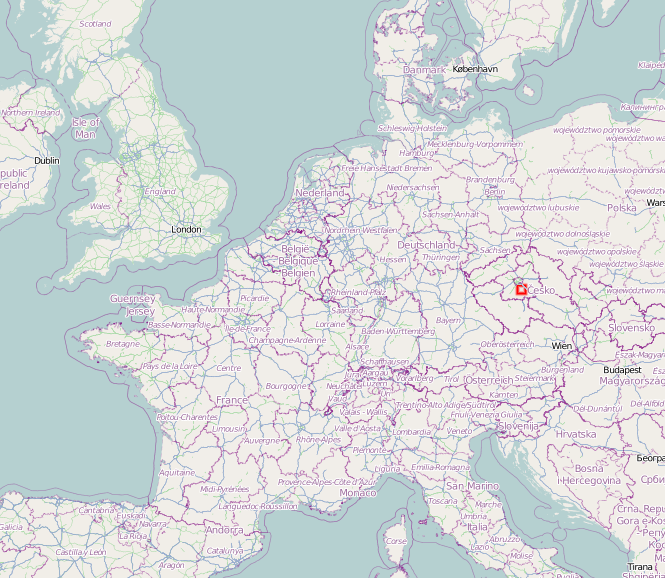
\includegraphics[width=\textwidth]{images/area.png}
    \end{column}
\end{columns}
\end{frame}

\begin{frame}{Disclamer}
\begin{block}{Disclamer}
    Numbers shown in this presentation are specific for used hardware, operating
    system, browser, position of stars and sun and other external conditions.

    \vskip5mm

    They are not meant to be taken as they are. They are here for illustration
    purpose, to demonstrate relative differences between various rendering
    techniques and libraries.
\end{block}
\end{frame}

\begin{frame}{Icons versus no-style}
\begin{center}
    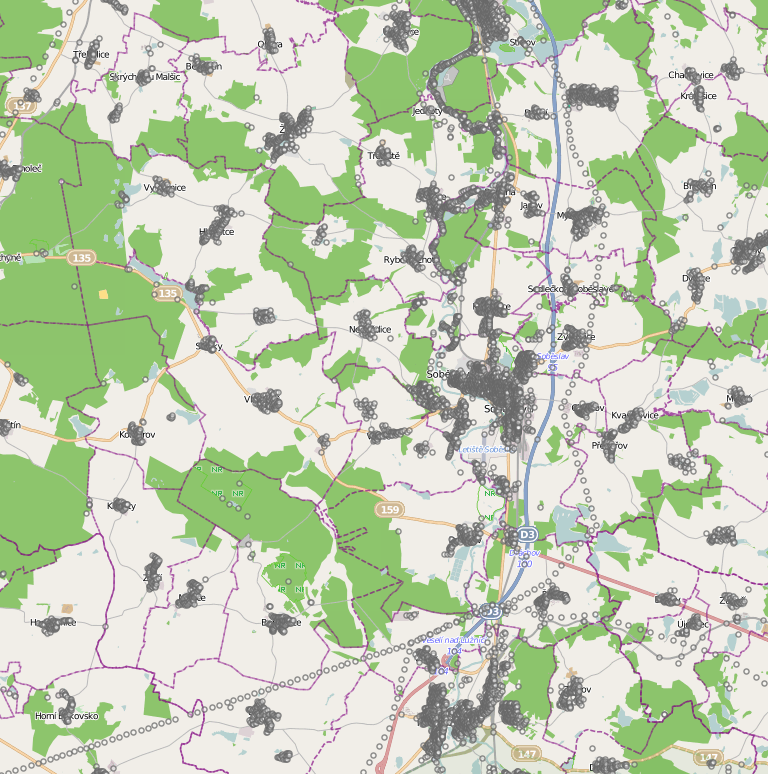
\includegraphics[width=0.45\textwidth]{images/no-style.png}~
    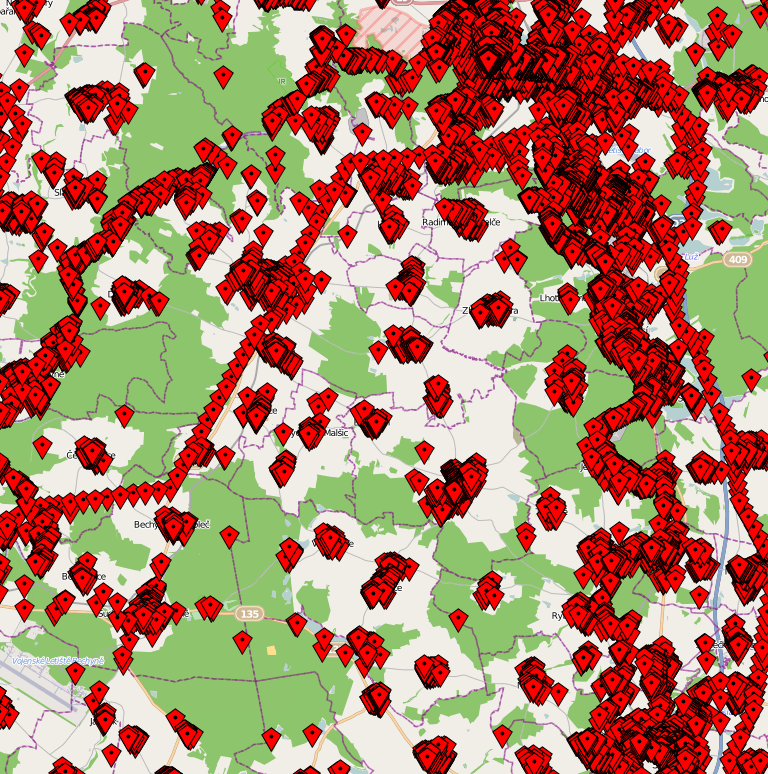
\includegraphics[width=0.45\textwidth]{images/icons.png}\\

    No-style versus image icons

\end{center}
\end{frame}

\mode<all>
\input{latexs/slides}

\begin{frame}{Result}
\begin{enumerate}[<+->]
    \item OpenLayers 3 Api Branch
    \item Leaflet 0.8-dev
    \item OpenLayers 2 Canvas
\end{enumerate}
\end{frame}

\section{Discussion}
\begin{frame}
\begin{itemize}[<+->]
    \item DOM vs. Canvas
    \item Image point icons versus no-style points
    \item Code / Speed ratio
    \item Parsing
    \item Bright future: WebGL
\end{itemize}
\end{frame}

\begin{frame}{DOM versus Canvas}
    \begin{center}
    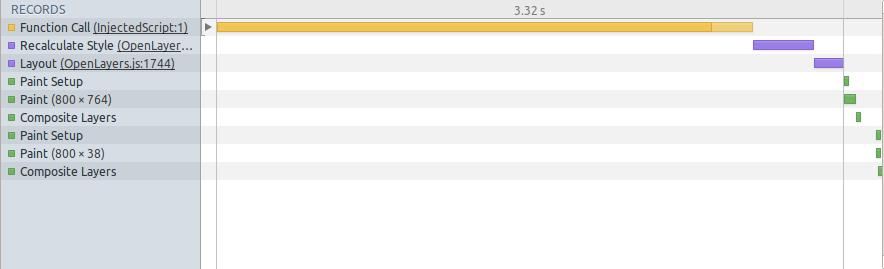
\includegraphics[width=\textwidth]{images/dom.png}\\
    DOM
    \\
    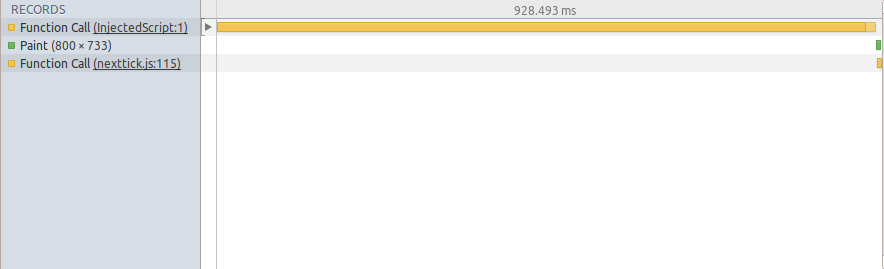
\includegraphics[width=\textwidth]{images/canvas.png}\\
    Canvas
    \end{center}
\end{frame}

\begin{frame}{Optimalizations}
\begin{itemize}[<+->]
    \item Data indexing
    \item Generalization
    \item Clustering
    \item Optimal rendering engine (DOM (SVG | VML) vs. Canvas vs. WebGL)
    \item Hardware improvements, browser improvements
\end{itemize}
\end{frame}


\section*{Conclusion}
\begin{frame}
    Happy web mapping!\\
    ~
    \\
    jachym.cepicky@gmail.com jachym.cepicky@geosense.cz\\
    http://les-ejk.cz http://geosense.cz\\
    @jachymc
\end{frame}


\end{document}
